\documentclass{article}
\usepackage[margin=1.0in]{geometry}
\usepackage{titling}
\usepackage{graphicx}
\usepackage{float}
\usepackage[T1]{fontenc}
\begin{document}
	
	%%% title
	\setlength{\droptitle}{-5em}
	\title{1.8 CPCTC - Corresponding Parts of Congruent Triangles are Congruent}
	\date{9/30/20}
	\author{}
	\maketitle
	
	%%% first section
	\section{CPCTC}
	
	Given $\triangle ABC \cong \triangle DEF $
	\newline 
	$\angle B \cong \angle E$
	\newline
	$\angle C \cong \angle D $
	\newline 
	$\angle A \cong \angle F$
	\newline \newline
	$AB \cong FE$, etc
	\newline
	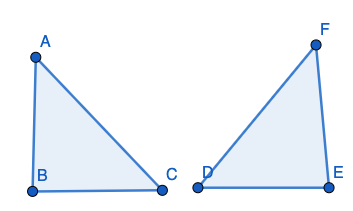
\includegraphics[scale=0.45]{pics/CPCTCex.png}
	
	
	\section{Medians}
	A segment drawn from a vertex to the \textbf{midpoint} of the opposite side
	\newline
	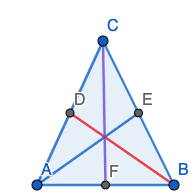
\includegraphics[scale=0.45]{pics/medians.png}
	
	
	\section{Altitude}
	A segment drawn from a vertex. Perpendicular on the opposite side.
	\newline
	\includegraphics[scale=0.45]{pics/altitude.png}
	
	
	\section{Auxiliary Line}
	A line added to a diagram (could be to enhance clarity)
\end{document}